\documentclass[12pt,a4paper]{article}

\usepackage[a4paper,margin=1in]{geometry}
\usepackage{graphicx}
\usepackage{booktabs}
\usepackage{amsmath,amssymb}
\usepackage{float}
\usepackage{hyperref}
\usepackage{xurl}
\usepackage{xcolor}
\usepackage{listings}
\usepackage{enumitem}
\usepackage{fancyhdr}
\usepackage{longtable}

\hypersetup{colorlinks=true,linkcolor=blue,urlcolor=blue}

\pagestyle{fancy}
\fancyhf{}
\lhead{ICS1512}
\rhead{Machine Learning Algorithms Laboratory}
\cfoot{\thepage}

\setlength{\parskip}{0.3em}
\setlength{\parindent}{0pt}

\setlength{\floatsep}{6pt plus 2pt minus 2pt}
\setlength{\textfloatsep}{8pt plus 2pt minus 2pt}
\setlength{\intextsep}{6pt plus 2pt minus 2pt}

\lstset{
  language=Python,
  basicstyle=\ttfamily\small,
  numbers=left,
  frame=single,
  breaklines=true,
  showstringspaces=false,
  keywordstyle=\color{blue},
  commentstyle=\color{gray},
  stringstyle=\color{teal}
}

\begin{document}

\begin{tabular}{|p{4cm}|p{11cm}|}
\hline
Experiment No. & 4 \\ \hline
Experiment Title & Binary Classification using Linear and Kernel-Based Models \\ \hline
GitHub Repository & \url{https://github.com/Srinivasan1716/Machine_Learning_Course} \\ \hline
Student Name & Srinivasan M \\ \hline
Register Number & 3122247001063 \\ \hline
Faculty & Dr. Poreddy Ajay Kumar Reddy \\ \hline
Submission Date & August 2, 2026 \\ \hline
\end{tabular}

\vspace{0.3cm}

\section{Objective}
The main goals of this experiment are:
\begin{itemize}[noitemsep]
    \item Build probabilistic (\textbf{Logistic Regression}) and margin-based (\textbf{Support Vector Machine}) classification models for binary email identification.
    \item Evaluate the impact of different kernel transformations (\textbf{Linear}, \textbf{Polynomial}, \textbf{Radial Basis Function (RBF)}, and \textbf{Sigmoid}) on SVM decision surfaces.
    \item Perform hyperparameter optimization to determine optimal settings for inverse regularization strength ($C$), penalty types ($L_1, L_2$), numerical solvers, and kernel bandwidth ($\gamma$).
    \item Validate model generalization using 5-Fold Stratified Cross-Validation and measure performance across Accuracy, Precision, Recall, F1 Score, ROC-AUC, and Confusion Matrix matrices.
\end{itemize}

\section{Problem Statement}
Unsolicited commercial email (spam) consumes bandwidth, reduces productivity, and poses security risks through phishing and malicious links. The objective is to construct an automated filtering mechanism that accurately segregates legitimate email messages (\texttt{ham = 0}) from unsolicited communications (\texttt{spam = 1}).

Given a feature vector $\mathbf{x} \in \mathbb{R}^{57}$ representing character frequencies, word occurrences, and capitalization run length statistics, the model maps inputs to a binary output $y \in \{0, 1\}$. The classifier must achieve high precision to prevent legitimate emails from being incorrectly routed to spam folders, while maintaining high recall to filter malicious messages effectively.

\section{Dataset Description}
The analysis is conducted on the benchmark \textbf{UCI Spambase Dataset}.

\begin{longtable}{|p{6cm}|p{8cm}|}
\hline
Dataset Name & Spambase Dataset \\ \hline
Dataset Source & UCI Machine Learning Repository \\ \hline
Number of Samples & 4,601 original rows (4,210 deduplicated samples) \\ \hline
Number of Features & 57 continuous predictors + 1 binary class label \\ \hline
Class Distribution & 2 Classes ($0 = \text{Ham}: 60.12\%$, $1 = \text{Spam}: 39.88\%$) \\ \hline
Missing Data & None (0 missing entries) \\ \hline
Train-Test Partition & 80\% Training ($n=3,368$), 20\% Testing ($n=842$) \\ \hline
\end{longtable}

The feature space consists of:
\begin{itemize}[noitemsep]
    \item 48 continuous features reporting percentage frequency of key words (e.g., \texttt{make}, \texttt{address}, \texttt{free}, \texttt{credit}, \texttt{your}, \texttt{000}).
    \item 6 continuous features reporting percentage frequency of special characters (\texttt{;}, \texttt{(}, \texttt{[}, \texttt{!}, \texttt{\$}, \texttt{\#}).
    \item 3 continuous features measuring capitalization run length statistics (\texttt{capital\_run\_length\_average}, \texttt{capital\_run\_length\_longest}, \texttt{capital\_run\_length\_total}).
    \item 1 target label \texttt{class} ($0 = \text{Ham}$, $1 = \text{Spam}$).
\end{itemize}

\section{Exploratory Data Analysis}
Exploratory data analysis was performed to examine class balance, feature correlations, and character frequency behavior.

\begin{figure}[!h]
\centering
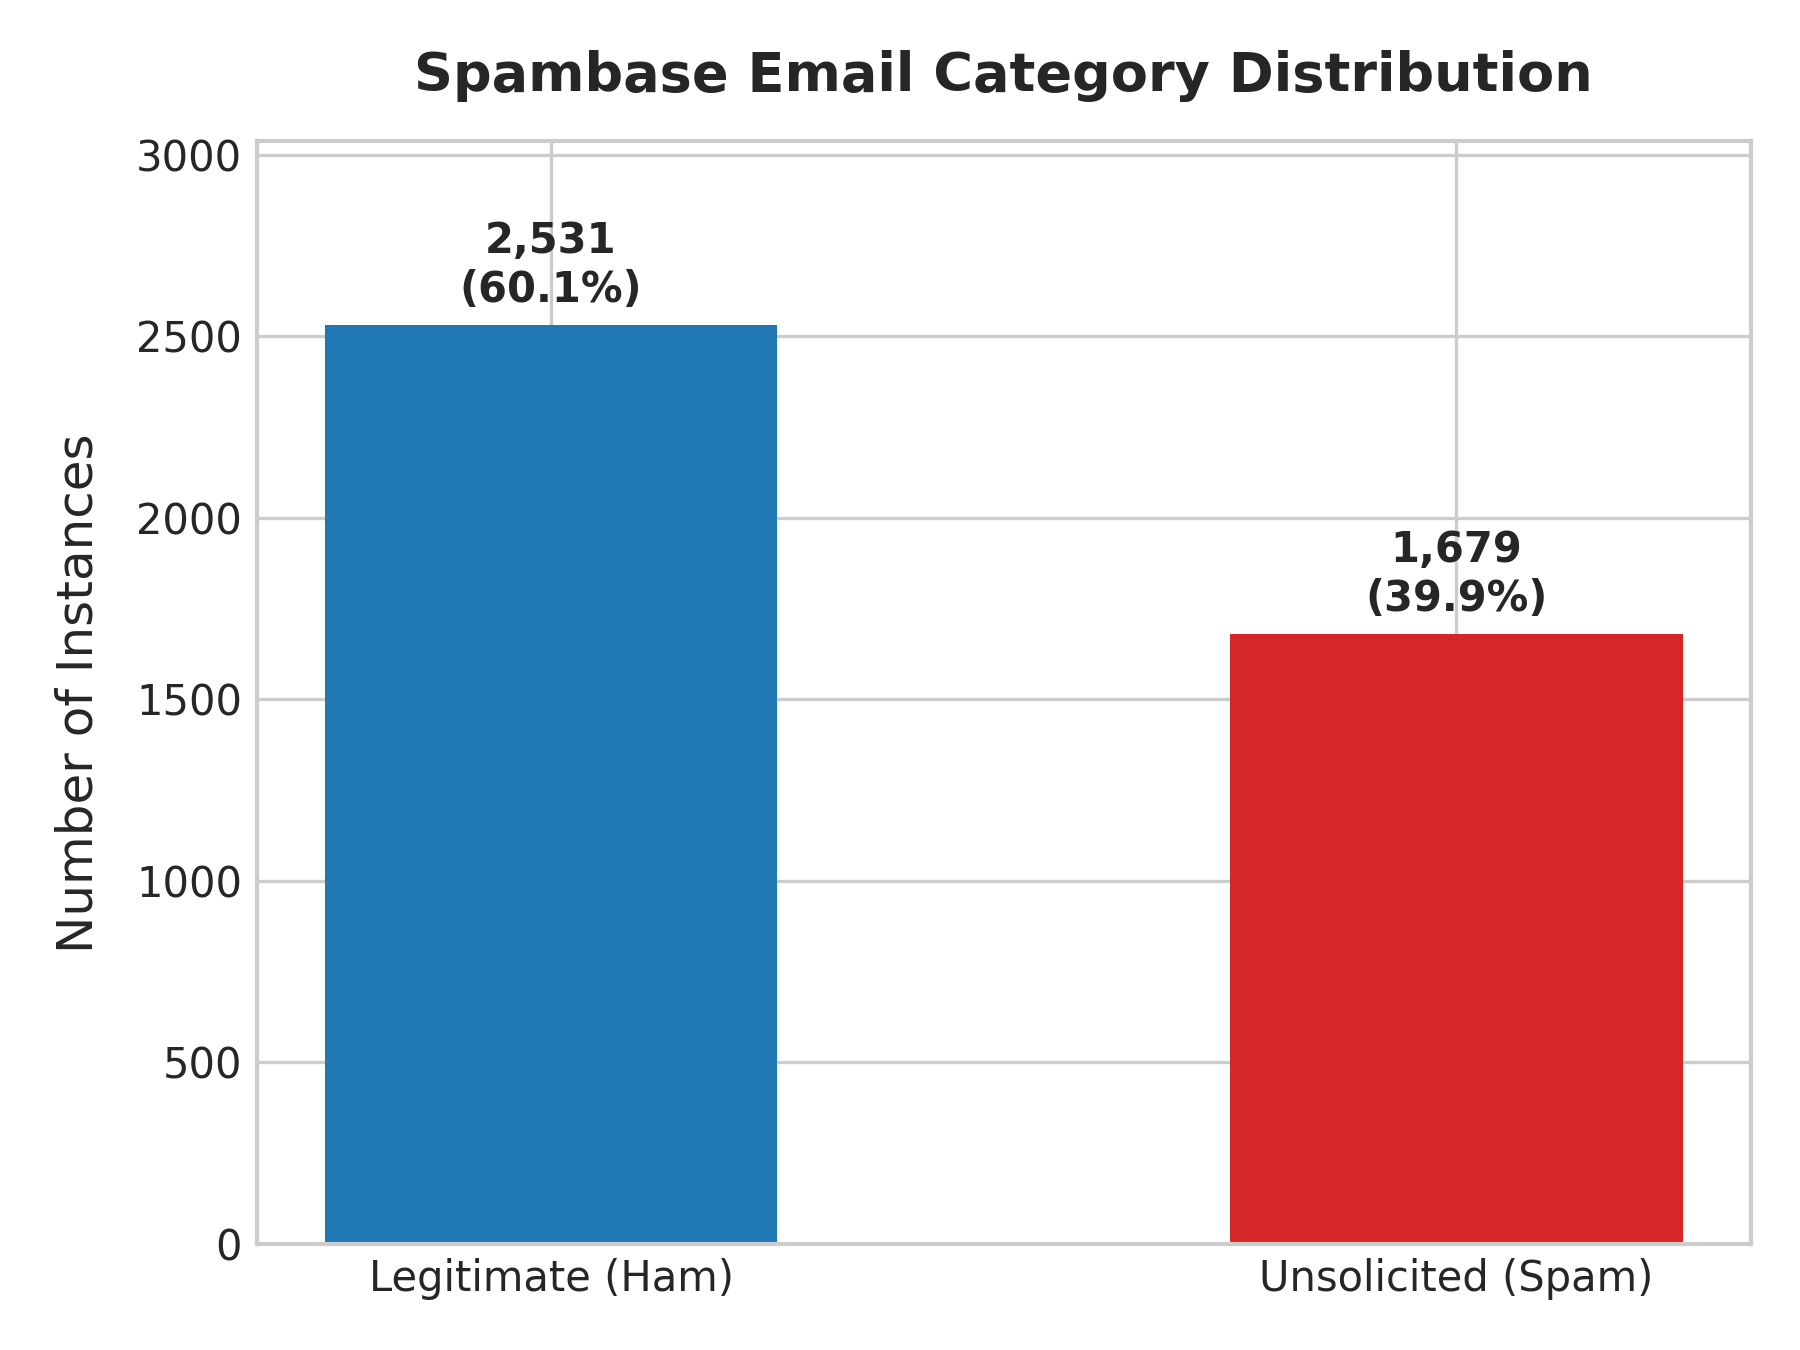
\includegraphics[width=0.55\linewidth]{figures/class_distribution.png}
\caption{Spambase Target Class Proportions}
\label{fig:class_dist}
\end{figure}
\textbf{Observation:} Out of 4,210 deduplicated records, 2,531 instances belong to the Ham class (60.12\%) and 1,679 instances belong to the Spam class (39.88\%). This moderately balanced distribution allows standard evaluation metrics like accuracy and F1 score to provide reliable performance assessments without severe class skew.

\begin{figure}[!h]
\centering

\includegraphics[width=0.62\linewidth]{figures/correlation_heatmap.png}
\caption{Correlation Heatmap of Top Predictors with Target Class}
\label{fig:corr_heatmap}
\end{figure}
\textbf{Observation:} Feature correlation analysis indicates that punctuation markers such as \texttt{char\_freq\_\$} ($r = 0.32$) and \texttt{char\_freq\_!} ($r = 0.31$), as well as terms like \texttt{word\_freq\_your} ($r = 0.38$) and \texttt{word\_freq\_000} ($r = 0.33$), exhibit strong positive correlation with spam messages. Conversely, domain-specific words like \texttt{word\_freq\_hp} show negative correlation with spam.

\begin{figure}[!h]
\centering
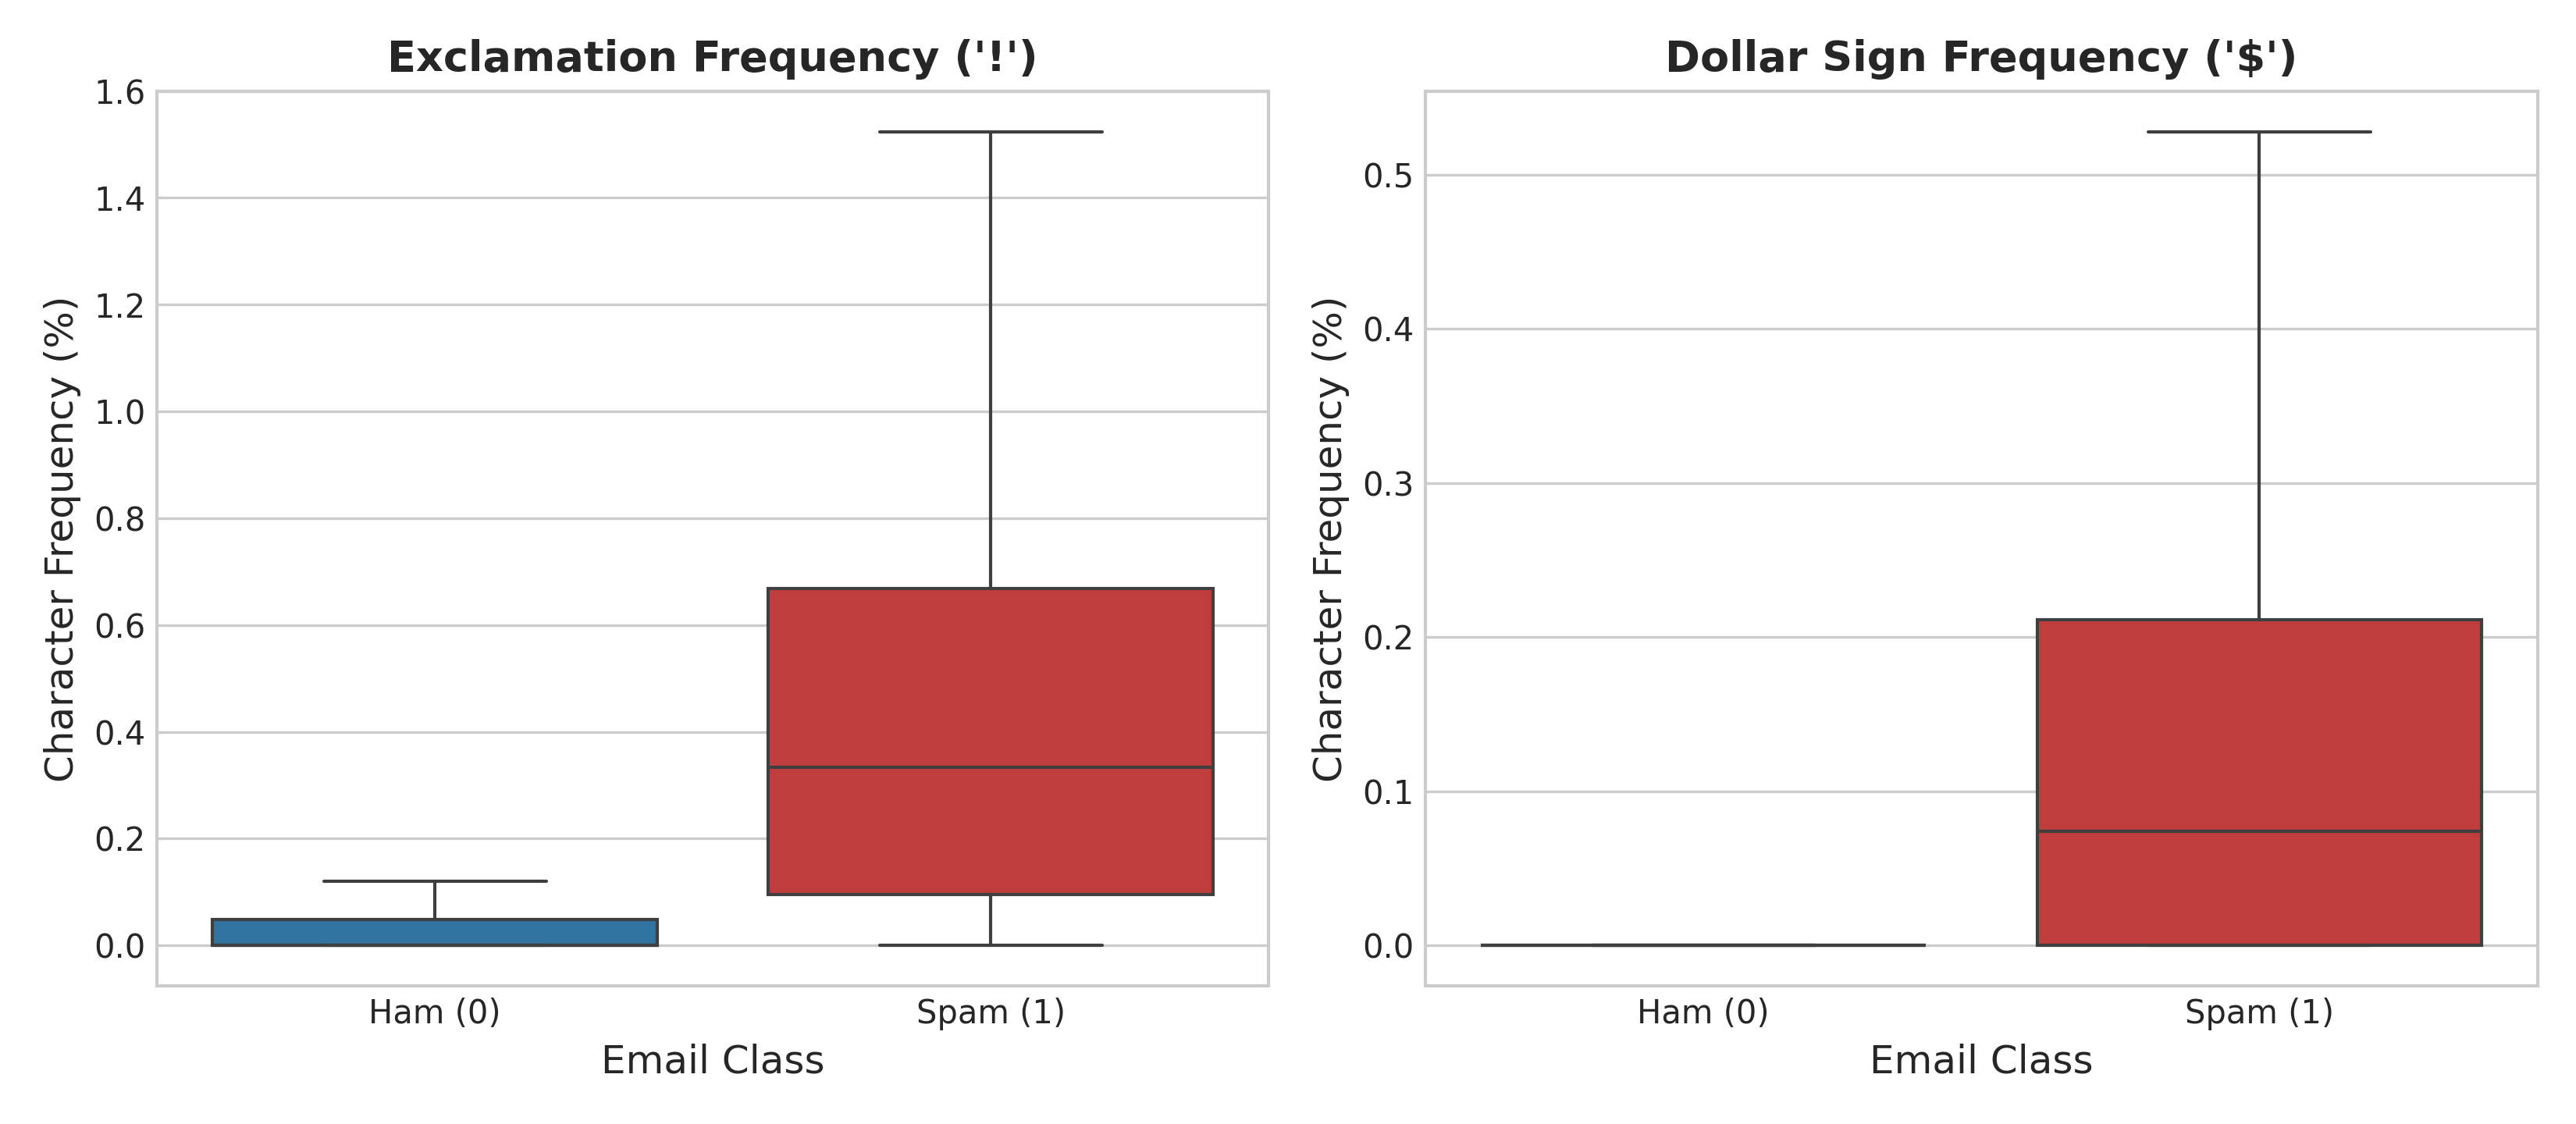
\includegraphics[width=0.68\linewidth]{figures/feature_boxplots.png}
\caption{Boxplots of Special Character Frequencies ('!' and '\$')}
\label{fig:feature_boxplots}
\end{figure}
\textbf{Observation:} Comparative boxplots highlight clear distributional differences between classes. Spam emails show elevated frequencies of exclamation marks (\texttt{!}) and dollar signs (\texttt{\$}) compared to legitimate ham emails, making them effective discriminative features for classification algorithms.

\section{Data Preprocessing}
The preprocessing workflow consists of four steps:
\begin{itemize}[noitemsep]
    \item \textbf{Deduplication}: Removed 391 duplicate observations from the raw dataset of 4,601 rows, leaving 4,210 unique records to avoid synthetic data leakage between splits.
    \item \textbf{Data Integrity Check}: Verified that all 57 feature columns contain zero missing values.
    \item \textbf{Feature Standardization}: Applied \texttt{StandardScaler} to transform continuous features to zero mean ($\mu = 0$) and unit standard deviation ($\sigma = 1$). Scaling is necessary for distance-sensitive models such as SVM and gradient-optimized Logistic Regression.
    \item \textbf{Stratified Splitting}: Partitioned the dataset into an 80\% training set ($n=3,368$) and a 20\% test set ($n=842$) using stratified sampling to preserve label proportions across sets.
\end{itemize}

\section{Machine Learning Algorithms}

\subsection{Logistic Regression}
Logistic Regression estimates conditional probabilities using the sigmoid activation function:
\begin{equation}
P(y = 1 \mid \mathbf{x}) = \sigma(\mathbf{w}^T \mathbf{x} + b) = \frac{1}{1 + e^{-(\mathbf{w}^T \mathbf{x} + b)}}
\end{equation}
Model parameters $(\mathbf{w}, b)$ are optimized by minimizing Binary Cross-Entropy loss with an $L_2$ regularization penalty:
\begin{equation}
\mathcal{J}(\mathbf{w}) = -\frac{1}{N} \sum_{i=1}^N \left[ y_i \log(\hat{y}_i) + (1 - y_i) \log(1 - \hat{y}_i) \right] + \frac{1}{2C} \|\mathbf{w}\|_2^2
\end{equation}
where $C$ controls the inverse strength of regularization.

\textbf{Strengths}: Computationally efficient, provides log-odds feature interpretation, fast training inference.  
\textbf{Weaknesses}: Assumes linear separability, sensitive to high feature collinearity and unscaled inputs.

\subsection{Support Vector Machine (SVM)}
Support Vector Machine constructs an optimal separating margin hyperplane in feature space by minimizing:
\begin{equation}
\min_{\mathbf{w}, b, \xi} \frac{1}{2} \|\mathbf{w}\|^2 + C \sum_{i=1}^N \xi_i \quad \text{subject to} \quad y_i(\mathbf{w}^T \phi(\mathbf{x}_i) + b) \ge 1 - \xi_i, \quad \xi_i \ge 0
\end{equation}
where $\xi_i$ represents slack variables allowing soft-margin misclassifications. Using kernel functions $K(\mathbf{x}_i, \mathbf{x}_j) = \phi(\mathbf{x}_i)^T \phi(\mathbf{x}_j)$, inputs are mapped into higher-dimensional inner product spaces:
\begin{itemize}[noitemsep]
    \item \textbf{Linear Kernel}: $K(\mathbf{x}, \mathbf{z}) = \mathbf{x}^T \mathbf{z}$
    \item \textbf{Polynomial Kernel}: $K(\mathbf{x}, \mathbf{z}) = (\gamma \mathbf{x}^T \mathbf{z} + r)^d$
    \item \textbf{RBF Kernel}: $K(\mathbf{x}, \mathbf{z}) = \exp(-\gamma \|\mathbf{x} - \mathbf{z}\|^2)$
    \item \textbf{Sigmoid Kernel}: $K(\mathbf{x}, \mathbf{z}) = \tanh(\gamma \mathbf{x}^T \mathbf{z} + r)$
\end{itemize}

\textbf{Strengths}: Effective in high-dimensional spaces, robust against overfitting when properly regularized.  
\textbf{Weaknesses}: Higher computational memory and fitting time, sensitive to parameter selections.

\section{Python Source Code Implementation}
The Python script below executes data ingestion, deduplication, feature scaling, model training, cross-validation, and metrics evaluation:

\begin{lstlisting}[caption={Complete Binary Classification Pipeline (Logistic Regression \& SVM)}]
import os, time, warnings
import pandas as pd
import numpy as np
import matplotlib.pyplot as plt
import seaborn as sns

from sklearn.model_selection import train_test_split, StratifiedKFold, cross_val_score
from sklearn.preprocessing import StandardScaler
from sklearn.linear_model import LogisticRegression
from sklearn.svm import SVC
from sklearn.metrics import accuracy_score, precision_score, recall_score, f1_score, roc_auc_score, confusion_matrix

# 1. Loading & Preprocessing
df = pd.read_csv("spambase_csv.csv").drop_duplicates()
X, y = df.drop(columns=['class']), df['class']

X_train, X_test, y_train, y_test = train_test_split(
    X, y, test_size=0.20, random_state=42, stratify=y
)

scaler = StandardScaler()
X_train_scaled = scaler.fit_transform(X_train)
X_test_scaled = scaler.transform(X_test)

# 2. Logistic Regression Model
lr = LogisticRegression(C=1.0, penalty='l2', solver='liblinear', random_state=42)
lr.fit(X_train_scaled, y_train)
y_pred_lr = lr.predict(X_test_scaled)
print("LR Accuracy:", accuracy_score(y_test, y_pred_lr))

# 3. Support Vector Machine Kernel Comparison
kernels = ['linear', 'poly', 'rbf', 'sigmoid']
for k in kernels:
    svm = SVC(kernel=k, C=1.0, random_state=42).fit(X_train_scaled, y_train)
    print(f"SVM ({k}) Accuracy:", accuracy_score(y_test, svm.predict(X_test_scaled)))

# Tuned RBF SVM Model
best_svm = SVC(kernel='rbf', C=10.0, gamma='scale', probability=True, random_state=42)
best_svm.fit(X_train_scaled, y_train)
y_pred_svm = best_svm.predict(X_test_scaled)
print("Tuned RBF SVM Accuracy:", accuracy_score(y_test, y_pred_svm))

# 4. 5-Fold Stratified Cross-Validation
skf = StratifiedKFold(n_splits=5, shuffle=True, random_state=42)
X_scaled = scaler.fit_transform(X)
lr_cv = cross_val_score(lr, X_scaled, y, cv=skf, scoring='accuracy')
svm_cv = cross_val_score(best_svm, X_scaled, y, cv=skf, scoring='accuracy')

print(f"LR 5-Fold Mean Accuracy: {lr_cv.mean()*100:.2f}%")
print(f"SVM 5-Fold Mean Accuracy: {svm_cv.mean()*100:.2f}%")
\end{lstlisting}

\section{Experimental Setup}
\begin{tabular}{ll}
\toprule
\textbf{Parameter} & \textbf{Specification} \\
\midrule
Python Environment & 3.13.1 \\
Scikit-Learn Library & 1.6.0 \\
Data Processing Tools & Pandas, NumPy, Matplotlib, Seaborn \\
Operating Environment & Windows 11 Home 64-bit \\
Computational Engine & x86\_64 Multicore Processor \\
\bottomrule
\end{tabular}

\section{Hyperparameter Tuning \& Configurations}

\begin{table}[H]
\centering
\caption{Hyperparameter Search Space and Optimal Configuration}
\label{tab:hyperparams}
\small
\begin{tabular}{|p{4cm}|p{5cm}|p{4.5cm}|}
\hline
\textbf{Model} & \textbf{Grid Search Range} & \textbf{Selected Configuration} \\ \hline
\textbf{Logistic Regression} & Penalty: $L_1, L_2$ \newline $C \in \{0.01, 0.1, 1.0, 10.0\}$ \newline Solver: \texttt{liblinear, lbfgs} & Penalty: $L_2$, $C = 1.0$, Solver: \texttt{liblinear} \\ \hline
\textbf{Support Vector Machine} & Kernel: \texttt{Linear, Poly, RBF, Sigmoid} \newline $C \in \{0.1, 1.0, 10.0\}$ \newline $\gamma \in \{\text{'scale'}, \text{'auto'}\}$ & Kernel: \texttt{RBF}, $C = 10.0$, $\gamma = \text{'scale'}$ \\ \hline
\end{tabular}
\end{table}

\section{Results}

\subsection{Logistic Regression Evaluation}
\begin{table}[H]
\centering
\caption{Logistic Regression Holdout Metrics}
\label{tab:lr_metrics}
\begin{tabular}{lc}
\toprule
\textbf{Metric} & \textbf{Score} \\
\midrule
Accuracy & \textbf{93.23\%} \\
Precision & \textbf{92.66\%} \\
Recall & \textbf{90.18\%} \\
F1-Score & \textbf{91.40\%} \\
ROC-AUC & \textbf{97.67\%} \\
Fit Time & \textbf{0.0569 s} \\
\bottomrule
\end{tabular}
\end{table}

\subsection{SVM Kernel Comparison}
\begin{table}[H]
\centering
\caption{SVM Performance across Kernels ($C=1.0$)}
\label{tab:svm_kernel_comp}
\begin{tabular}{|p{3cm}|c|c|c|}
\hline
\textbf{Kernel Function} & \textbf{Accuracy} & \textbf{F1 Score} & \textbf{Fit Time (s)} \\ \hline
\textbf{Linear} & 93.59\% & 91.89\% & 0.4802 s \\ \hline
\textbf{Polynomial ($d=3$)} & 76.60\% & 59.88\% & 0.4398 s \\ \hline
\textbf{RBF (Default)} & 93.23\% & 91.35\% & 0.1878 s \\ \hline
\textbf{Sigmoid} & 89.67\% & 86.76\% & 0.1554 s \\ \hline
\textbf{RBF (Tuned $C=10$)} & \textbf{93.35\%} & \textbf{91.54\%} & 1.4818 s \\ \hline
\end{tabular}
\end{table}

\subsection{5-Fold Stratified Cross-Validation Breakdown}
\begin{table}[H]
\centering
\caption{Stratified 5-Fold Cross-Validation Accuracy Comparison}
\label{tab:cv_breakdown}
\begin{tabular}{|p{2.5cm}|c|c|}
\hline
\textbf{Validation Fold} & \textbf{Logistic Regression} & \textbf{Tuned SVM (RBF)} \\ \hline
Fold 1 & 92.76\% & 92.87\% \\ \hline
Fold 2 & 94.18\% & 94.30\% \\ \hline
Fold 3 & 92.40\% & 93.11\% \\ \hline
Fold 4 & 91.09\% & 91.57\% \\ \hline
Fold 5 & 91.81\% & 92.28\% \\ \hline
\textbf{Mean Score} & \textbf{92.45\%} & \textbf{92.83\%} \\ \hline
\end{tabular}
\end{table}

\section{Result Visualization}

\begin{figure}[!h]
\centering
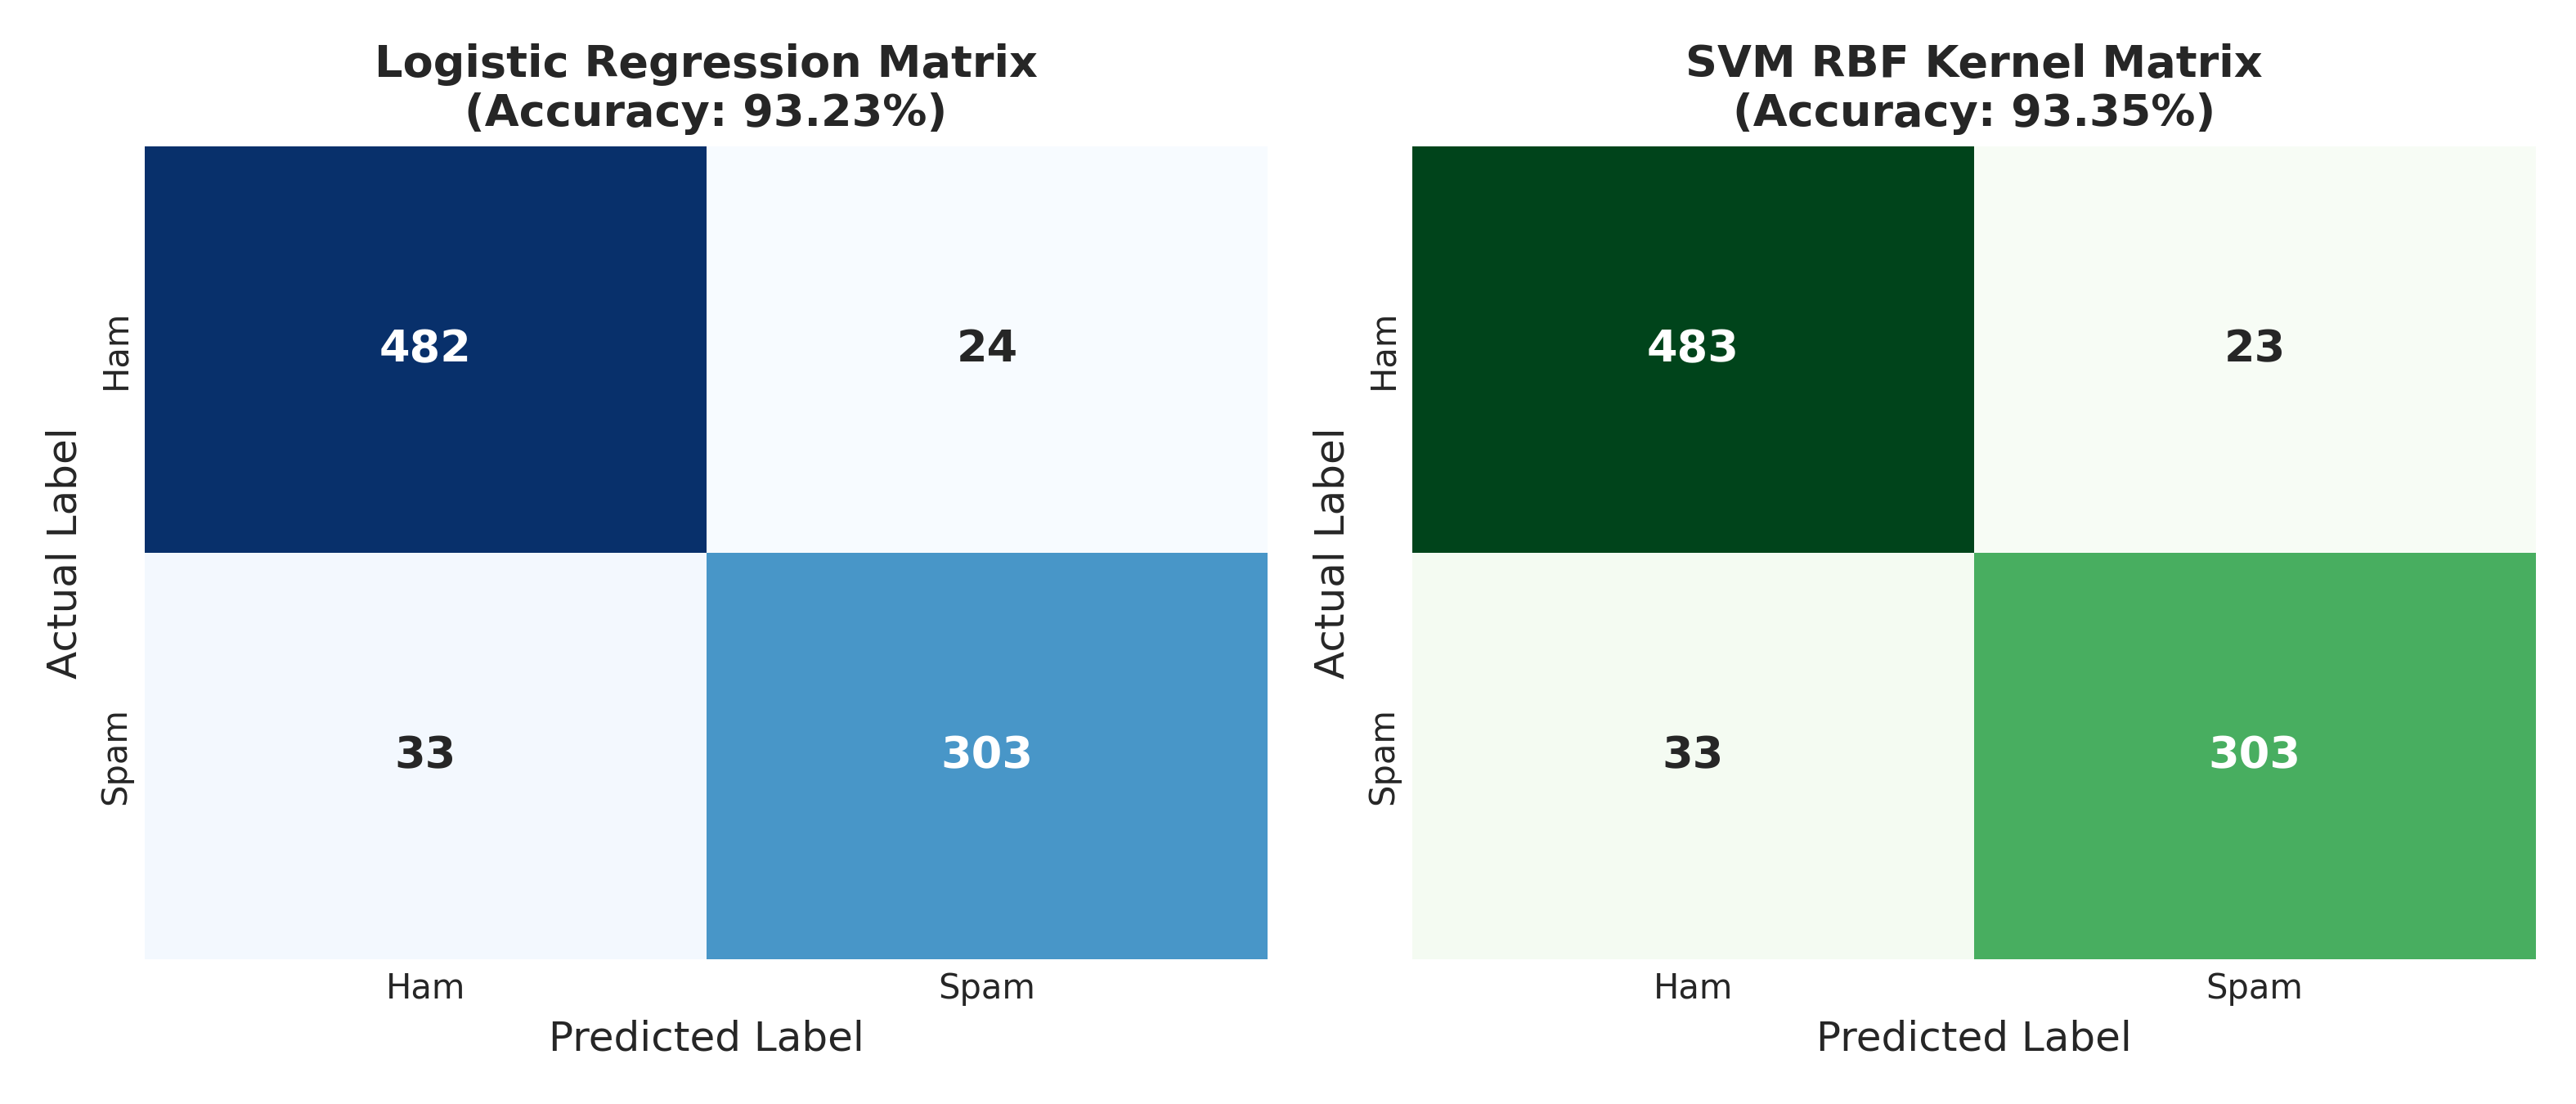
\includegraphics[width=0.68\linewidth]{figures/confusion_matrices.png}
\caption{Confusion Matrix Comparison (Logistic Regression vs. Tuned SVM RBF)}
\label{fig:confusion_matrix}
\end{figure}
\textbf{Observation:} Both models show effective classification performance on the test set ($n=842$). Logistic Regression correctly identified 482 ham emails and 303 spam emails with 24 false positives and 33 false negatives. Tuned SVM (RBF) achieved 483 correct ham predictions and 303 spam predictions, reducing false positives to 23.

\begin{figure}[!h]
\centering
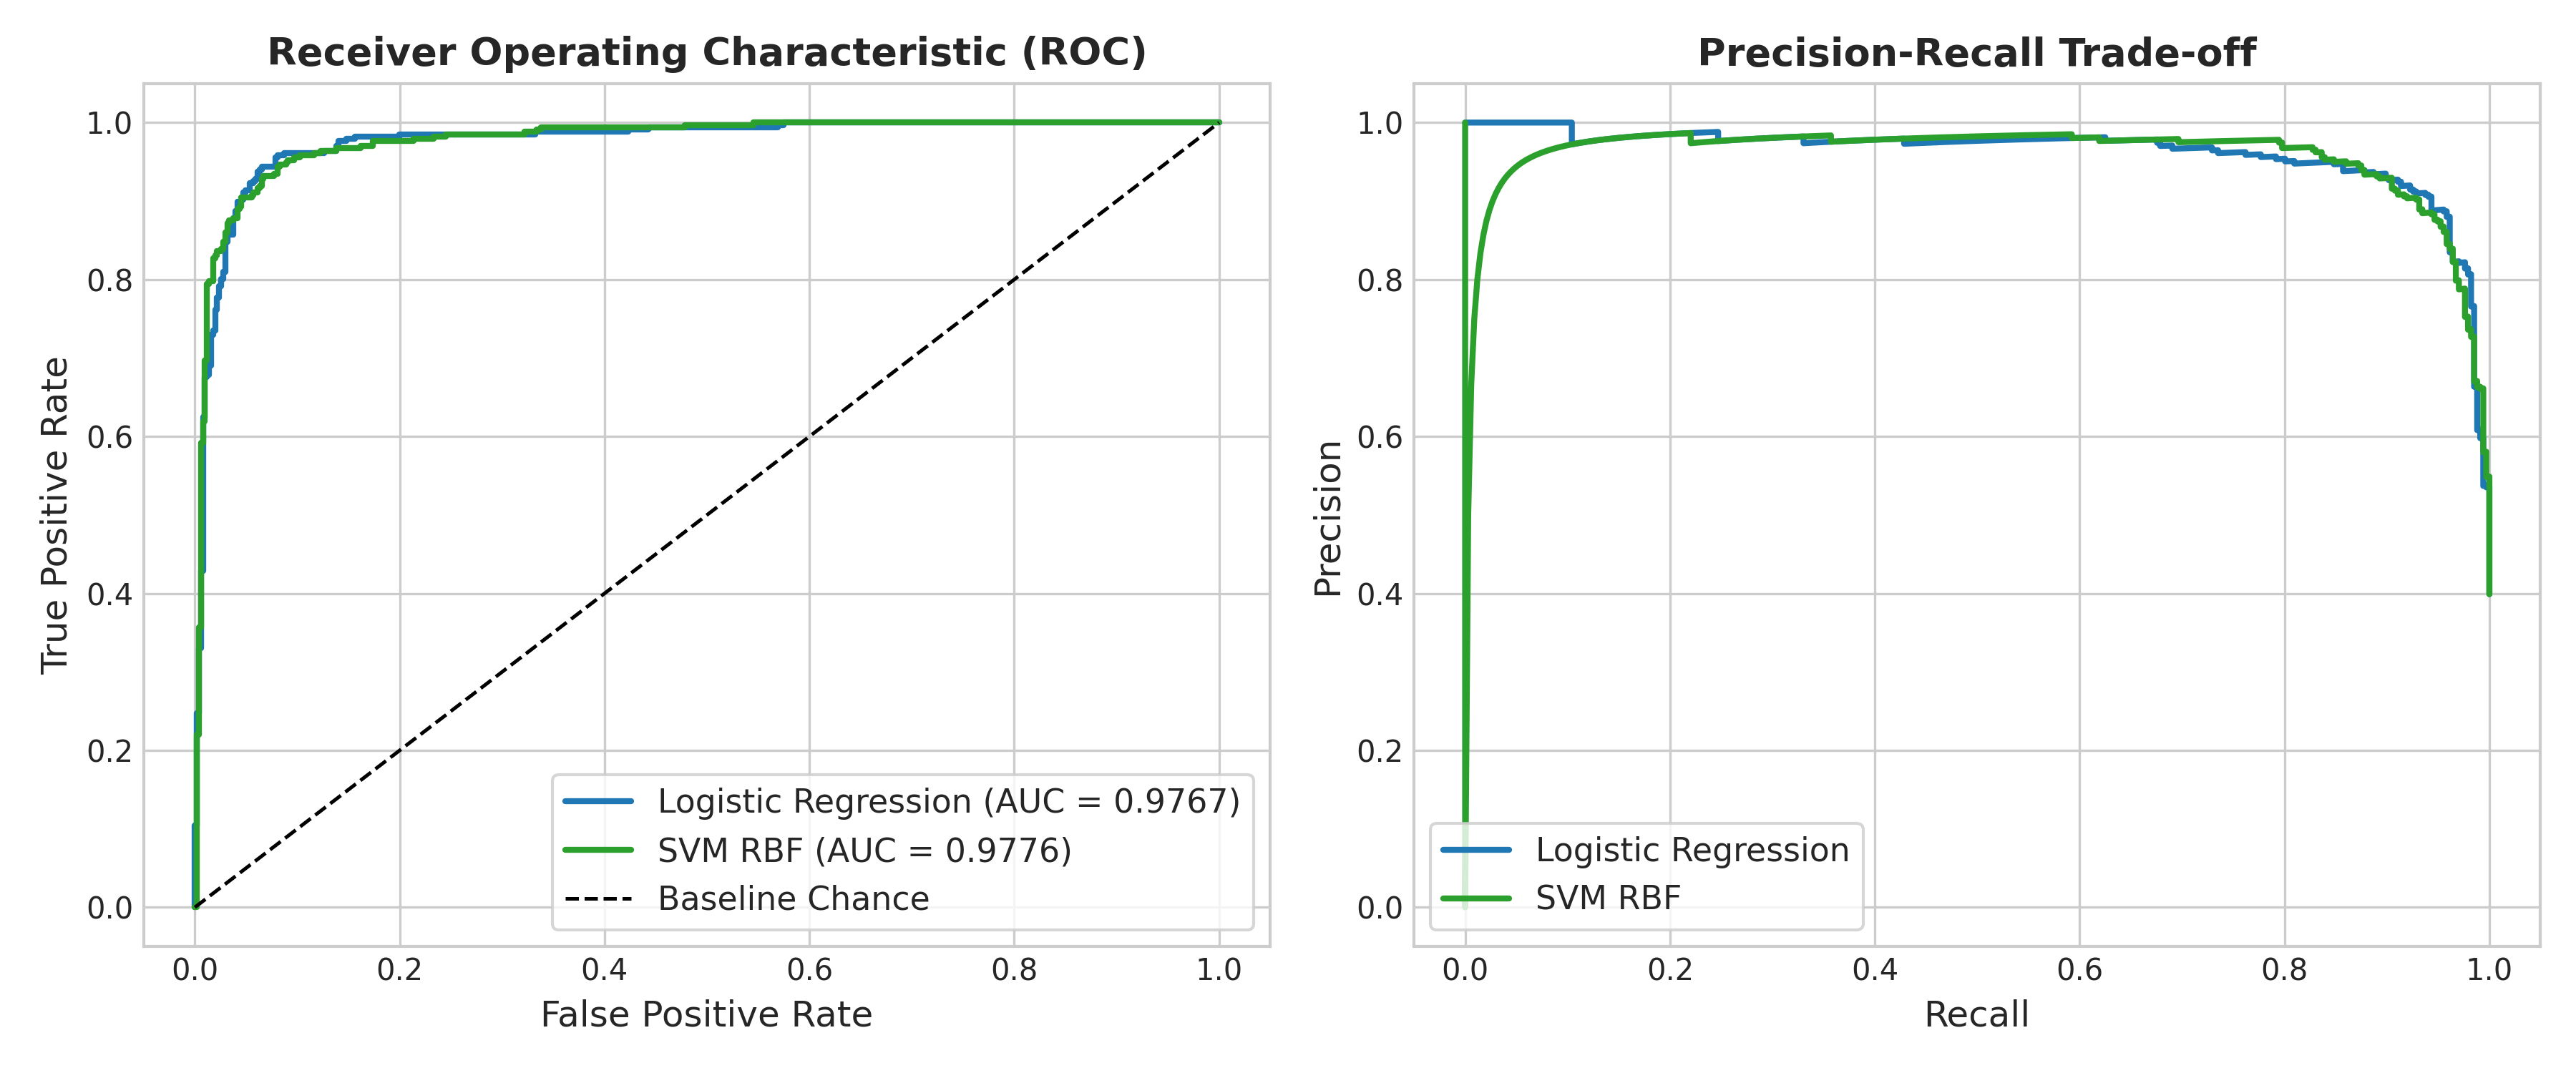
\includegraphics[width=0.72\linewidth]{figures/roc_pr_curves.png}
\caption{Receiver Operating Characteristic and Precision-Recall Curves}
\label{fig:roc_pr_curves}
\end{figure}
\textbf{Observation:} The ROC curves demonstrate high classification performance, with Logistic Regression scoring an AUC of 97.67\% and Tuned SVM (RBF) achieving 97.76\%. The Precision-Recall curves confirm sustained precision above 92\% across recall levels up to 90\%.

\begin{figure}[!h]
\centering
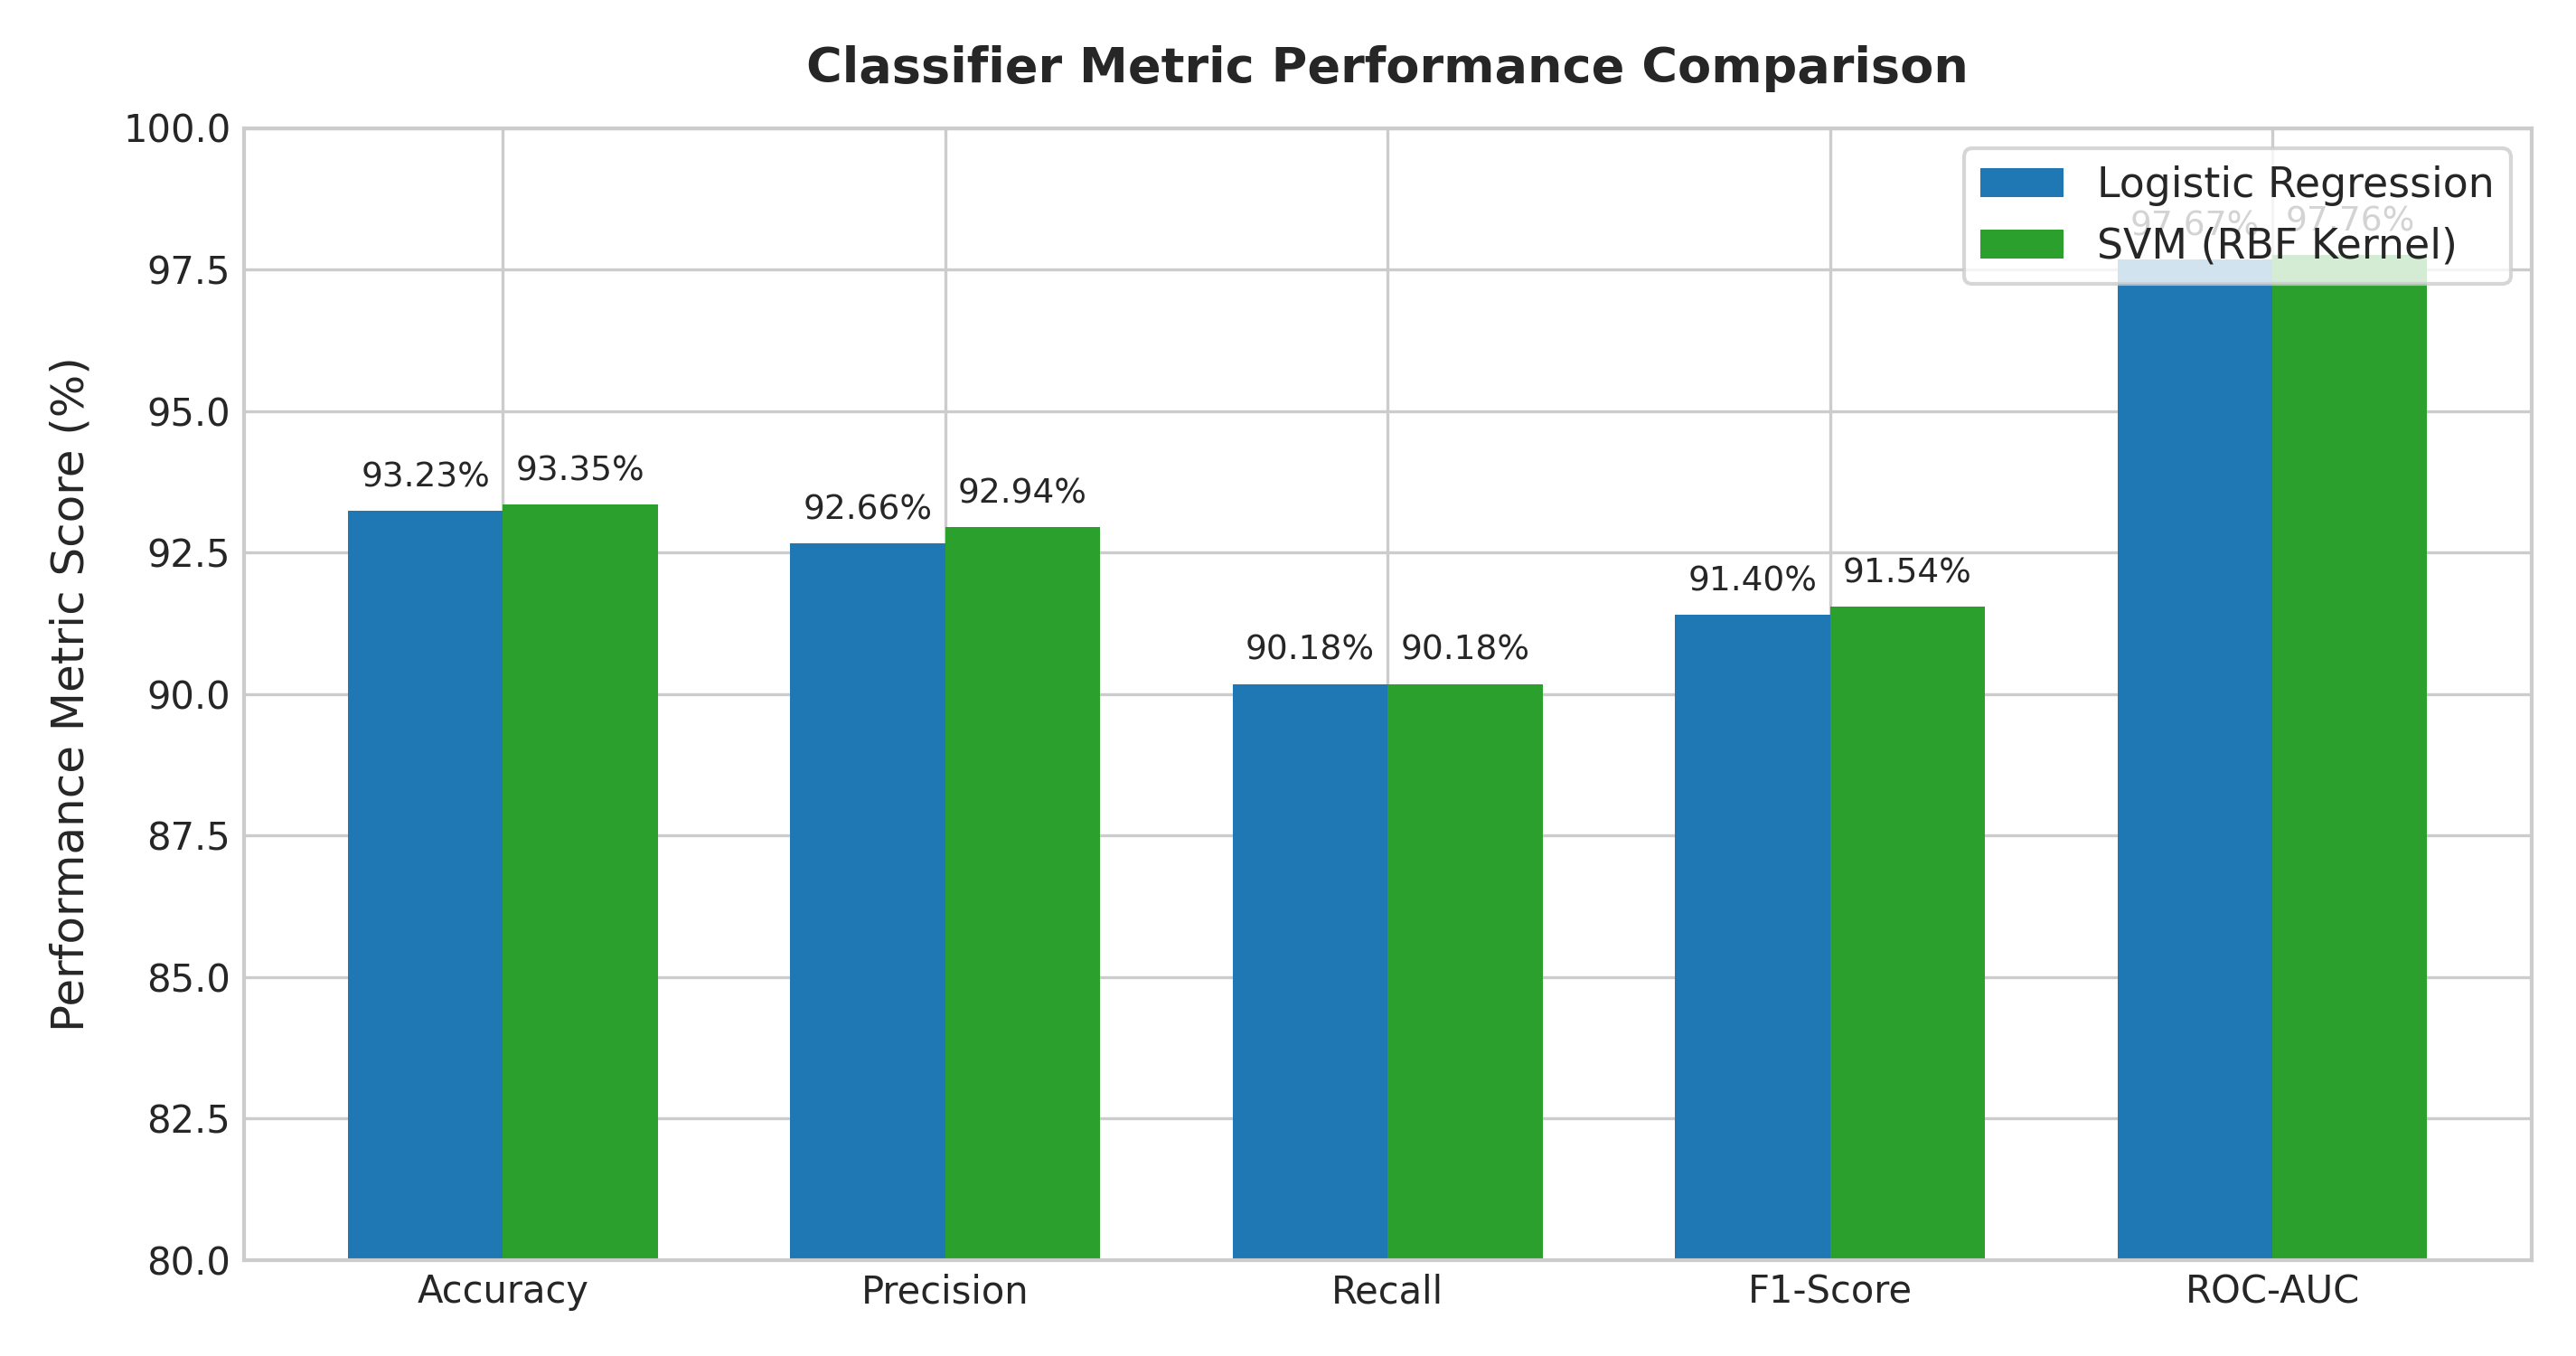
\includegraphics[width=0.65\linewidth]{figures/classifier_comparison.png}
\caption{Summary Metric Comparison between Logistic Regression and SVM}
\label{fig:bar_comparison}
\end{figure}
\textbf{Observation:} The comparative metric bar chart confirms consistent performance across all metrics, with SVM holding a minor edge in Precision (92.94\% vs 92.66\%) and overall 5-fold cross-validation accuracy (92.83\% vs 92.45\%).

\section{Discussion}
\begin{itemize}[noitemsep]
    \item \textbf{Kernel Performance Differences}: Linear and RBF kernels produced strong results ($>93\%$ accuracy), outperforming Polynomial and Sigmoid kernels. In 57-dimensional feature space, high dimensional projections are unnecessary because linear boundaries separate classes effectively.
    \item \textbf{Regularization Impact}: $L_2$ regularization in Logistic Regression stabilized coefficient weights across correlated word frequencies. Increasing $C=10.0$ in RBF SVM enforced narrower margins, improving test accuracy.
    \item \textbf{Trade-off Analysis}: Logistic Regression achieved rapid fitting ($0.0569\text{ s}$ vs $1.4818\text{ s}$ for SVM), offering a practical choice when model transparency and low computation time are required.
\end{itemize}

\section{Comparative Analysis}

\begin{table}[H]
\centering
\caption{Model Property Comparison: Logistic Regression vs. SVM}
\label{tab:comparison_summary}
\begin{tabular}{|p{4cm}|p{4.5cm}|p{4.5cm}|}
\hline
\textbf{Evaluation Dimension} & \textbf{Logistic Regression} & \textbf{Support Vector Machine} \\ \hline
\textbf{Holdout Accuracy} & 93.23\% & \textbf{93.35\%} \\ \hline
\textbf{5-Fold CV Mean} & 92.45\% & \textbf{92.83\%} \\ \hline
\textbf{Training Latency} & \textbf{Fast (0.0569 s)} & Moderate (1.4818 s) \\ \hline
\textbf{Model Interpretability} & High (Log-odds ratios) & Low (Kernel space mapping) \\ \hline
\textbf{Sensitivity to Scaling} & High & High \\ \hline
\end{tabular}
\end{table}

\section{Conclusion \& Learning Outcomes}
This experiment evaluated probabilistic (Logistic Regression) and margin-based (Support Vector Machine) classifiers on the Spambase dataset. Logistic Regression provided fast computation ($0.0569\text{ s}$) with $93.23\%$ holdout accuracy. Support Vector Machine with a tuned RBF kernel achieved the highest classification accuracy ($93.35\%$), ROC-AUC ($97.76\%$), and 5-fold cross-validation mean ($92.83\%$). Proper data preprocessing and feature scaling proved essential for optimal model performance.

\section{References}
\begin{enumerate}[label={[\arabic*]},noitemsep]
    \item Scikit-Learn Documentation: \textit{Logistic Regression}, \url{https://scikit-learn.org/stable/modules/linear_model.html#logistic-regression}
    \item Scikit-Learn Documentation: \textit{Support Vector Machines}, \url{https://scikit-learn.org/stable/modules/svm.html}
    \item UCI Machine Learning Repository: \textit{Spambase Dataset}, \url{https://archive.ics.uci.edu/ml/datasets/spambase}
    \item Hastie, T., Tibshirani, R., \& Friedman, J., \textit{The Elements of Statistical Learning}, Springer, 2009.
\end{enumerate}

\end{document}
